% This file provides the generic header that sets up the page formatting and
% common custom macro and environment definitions that will be used for the
% C and C++ programming course.
%
% You can consult the `00-Example_Usage.tex` file for a full example of how to
% use this header file.
%

% The documentclass is set to an a4 paper article using KOMA-script
\documentclass[paper=a4]{scrartcl}
\PassOptionsToPackage{hyphens}{url}
\setlength\parindent{0pt}

% Hyperref is used, allowing for linking between different parts of the pdf.
\usepackage[breaklinks=true,colorlinks=true,linkcolor=red]{hyperref}
\hypersetup{urlcolor=red}
\def\UrlFont{\em}
\usepackage{attachfile}
\usepackage[utf8]{inputenc}
% Geometry sets the exact dimensions of the page, overriding KOMA-scripts DIM.
\usepackage[top=0.5in,bottom=1in,left=0.5in,right=0.5in]{geometry}

% Tabu provides better tables than the built in tabular environment.
\usepackage{tabu}

% Allows us to use the H param for exact figure placement
\usepackage{float}
% Provides todos
\usepackage{todonotes}
\newcommand{\jk}[1]{\todo[inline,color=green]{JK: #1}}
\newcommand{\llb}[1]{\todo[inline,color=blue!20]{LLB: #1}}
\newcommand{\ob}[1]{\todo[inline,color=red!20]{OB: #1}}

% Adds additional section configuration options, these mirror `\date` and
% `\author` in behaviour.
\usepackage{totcount}
\makeatletter
\newcounter{cs@exercise}
\newcommand{\exercise}[1]{\setcounter{cs@exercise}{#1}}
\newcommand{\theexercise}{\arabic{cs@exercise}}
\newcounter{cs@xmarks}
\regtotcounter{cs@xmarks}
\newcommand{\totalxmarks}{\total{cs@xmarks}}
\newcommand{\addxmark}[1]{\addtocounter{cs@xmarks}{#1}}
\newcounter{cs@minutes}
\regtotcounter{cs@minutes}
\newcommand{\totalminutes}{\total{cs@minutes}}
\newcommand{\addminutes}[1]{\addtocounter{cs@minutes}{#1}}
\newtoks{\internal@term}
\newcommand{\term}[1]{\internal@term={#1}}
\newcommand{\theterm}{\the\internal@term}
\makeatother

% The following are used to configure the footer of the document.
\usepackage{lastpage}
\usepackage{fancyhdr}
\usepackage{titling}
\usepackage{textcomp}
\pagestyle{fancy}
\fancyhf{}
\rhead{}
\lhead{}
\lfoot{Visit Day Tutorial}
\cfoot{\today}
\rfoot{\thepage/\pageref{LastPage}}

% Listings is used for the inclusion of source code.
\usepackage{xcolor}
\usepackage{textcomp} %for upquote=true (straight quotes)
\usepackage{listings}
\definecolor{pblue}{rgb}{0.13,0.13,1}
\definecolor{pgreen}{rgb}{0,0.5,0}
\definecolor{pred}{rgb}{0.9,0,0}
\definecolor{pgrey}{rgb}{0.46,0.45,0.48}

\lstdefinelanguage{JavaScript}{
  keywords={typeof, new, true, false, catch, function, return, null, catch, switch, var, if, in, while, do, else, case, break},
  keywordstyle=\color{blue}\bfseries,
  ndkeywords={class, export, boolean, throw, implements, import, this},
  ndkeywordstyle=\color{darkgray}\bfseries,
  identifierstyle=\color{black},
  sensitive=false,
  comment=[l]{//},
  morecomment=[s]{/*}{*/},
  commentstyle=\color{purple}\ttfamily,
  stringstyle=\color{red}\ttfamily,
  morestring=[b]',
  morestring=[b]"
}

\lstset{
	basicstyle=\ttfamily\footnotesize,
	numberstyle=\ttfamily\tiny,
	frame=single,
	numbers=left,
	numbersep=1em,
	xleftmargin=2em,
	language=Javascript,
	breaklines=true,
	breakatwhitespace=true,
	postbreak=\hbox{$\hookrightarrow$ },
	showstringspaces=false,
	tabsize=2,
	commentstyle=\color{pgreen},
	keywordstyle=\color{pblue},
	stringstyle=\color{pred},
	moredelim=[il][\textcolor{pgrey}]{\[\]},
	moredelim=[is][\textcolor{pgrey}]{\%\%}{\%\%},
  columns=fullflexible,
	upquote=true
}
\usepackage{cleveref}

\parskip 8pt

\term{Spring 2021}

% The following defines the command \makesheetheader which is used to create
% the header shown at the top of every exercise sheet.
\definecolor{infobox}{HTML}{e0f7fa}
\newcommand{\makesheetheader}{%
    \thispagestyle{empty}
    \begin{center}
    	\begin{tabular*}{\textwidth}{@{}l@{\extracolsep{\fill}}r@{}}
    	  University of Reading & Tutorial Visit Day \\
    		Department of Computer Science	&  / \theterm \\
        \theauthor     & \totalminutes{} Minutes \\
    		\hline
    	\end{tabular*}
    \end{center}%
}

% The `submissions` Environment is used for listing the work outputs expected to
% be produced for any given exercise.

\newlinechar=`\^^J


% The following commands are used to declare the starts of each section, with how long they are expected to take and how many marks are expected if any.
\newcommand{\generaltoc}[2]{%
	\addtocounter{section}{1}%
	\section*{\arabic{section}. #2: #1}%
	\addcontentsline{toc}{section}{\arabic{section}. #2: #1}%
	\setcounter{subsection}{0}
}
\newcommand{\tutorial}[2]{%
		\generaltoc{#1}{Tutorial (#2 Minutes)}%
		\addminutes{#2}%
}
\newcommand{\markedtutorial}[3]{%
    \generaltoc{#1}{Marked Tutorial (#2 Minutes, #3 Marks)}%
    \addminutes{#2}%
    \addxmark{#2}%
}
\newcommand{\groupwork}[2]{%
    \generaltoc{#1}{Group Work (#2 Minutes)}%
    \addminutes{#2}%
}
\newcommand{\markedgroupwork}[3]{%
    \generaltoc{#1}{Marked Group Work (#2 Minutes, #3 Marks)}
    \addminutes{#2}%
    \addxmark{#3}%
}

% The following define reusable subsections.
\newenvironment{critera}{%
    \subsection*{Marking Criteria}
    \begin{itemize}
}{%
    \end{itemize}
}
\newenvironment{criteria*}{
    \subsection*{Marking Criteria}
}{}
\newenvironment{steps}{%
    \subsection*{Steps}
    \begin{enumerate}
}{%
    \end{enumerate}
}
\newenvironment{steps*}{
    \subsection*{Steps}
}{}
\newenvironment{literature}{%
    \subsection*{Further Reading}
    \begin{itemize}
}{
    \end{itemize}
}
\newenvironment{literature*}{
    \subsection*{Further Reading}
}{}
\newenvironment{hints}{%
    \subsection*{Hints}
    \begin{itemize}
}{
    \end{itemize}
}
\newenvironment{hints*}{
    \subsection*{Hints}
}{}
% These are not currently used, and if the previous definitions were anything
% to go by should likely be replaced by environments also.
% \newcommand{\Input}{\subsection*{Input}}
% \newcommand{\Output}{\subsection*{Output}}
% \newcommand{\example}{\subsection*{Example}}

\newcommand{\cmd}[1]{\texttt{\$~#1}}
\newcommand{\func}[1]{\texttt{#1()}}


\begin{document}

\author{Julian Kunkel}

\makesheetheader
\parskip 8pt

\textit{%
This tutorial is an example from the Computer Science module Programming in C/C++, which is a first year module. It demonstrates how the lab practicals are organized:
\begin{itemize}
  \item Lectures deliver theoretical knowledge.
  \item Lab practicals apply the theory in practice and provide training for skills such as programming.
  \item In the Programming module, lab practicals use tutorials consisting of individual work and group work.
\end{itemize}
}

\textit{%
If you were a first year student taking the Programming module,
by this point, you would already have been given additional exercises to help you practise the basics before attempting these tasks.
For this session, though, we have decided to jump straight into the more interesting part of the practical.
}

\textbf{If you have any questions, we encourage you to attract the attention of the lecturer or the assistants, for example, by raising your hand.}

\section*{Learning Objectives}

By the end of the tutorial, you will be able to:

\begin{itemize}
  \item Use Visual Studio to execute and modify a program.
  \item Describe the behaviour of the structured programming theorem constructs (sequence, selection, iteration).
\end{itemize}

\tableofcontents

\clearpage

\tutorial{Compiling a Program using Visual Studio}{20}

As part of this tutorial, we will use Visual Studio to download, modify and build an existing program.

\begin{steps}
  \item In the Start menu, search for and start \textbf{Microsoft Visual Studio}.
  Once Visual Studio is loaded, if you are asked whether you want to "Connect to all your developer services", select: "Not now, maybe later" at the bottom.
  You may have to confirm again to start the program.
  % also Start visual studio
  You will then be presented with the opening splash screen:

  \begin{figure}[H]
      \centering
      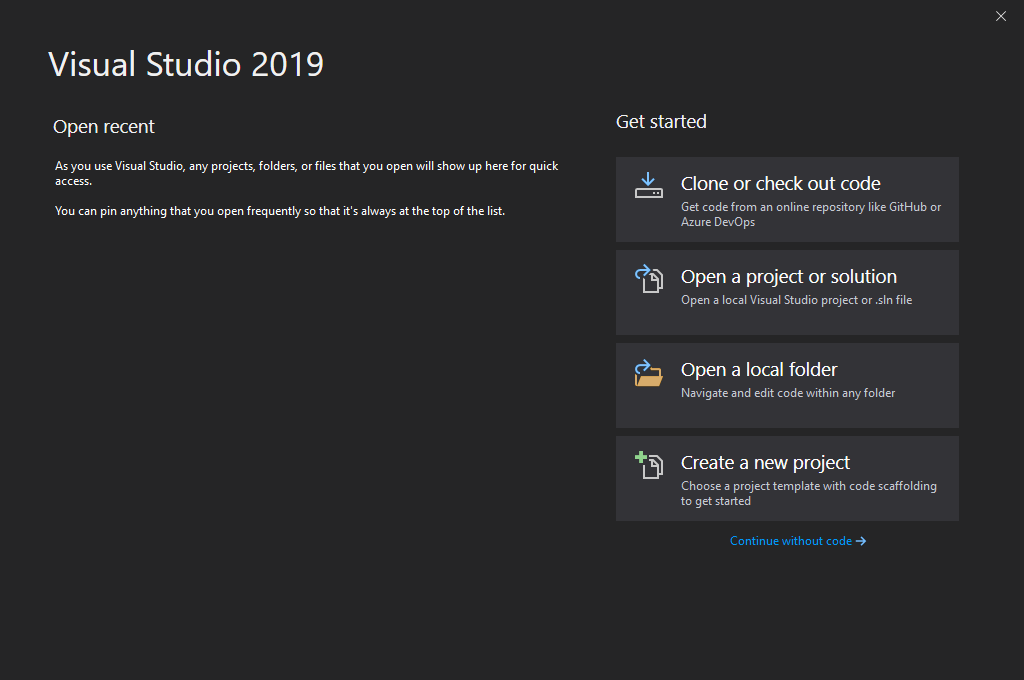
\includegraphics[width=0.8\textwidth]{img/splash.png}
      \caption{\label{splash} Microsoft Visual Studio Splash Launcher}
  \end{figure}

  \item Select “Clone or check out code”.
  \item Input the URL: \url{https://csgitlab.reading.ac.uk/di918039/visitday.git} and confirm.
  \item Next, we will look at the basics of Visual Studio to understand the Main Editor and Solution Explorer. \\
  Have a look at \url{https://docs.microsoft.com/en-us/visualstudio/get-started/visual-studio-ide?view=vs-2019} in a web browser.
  \item In the \textbf{Solution Explorer}, select the file {\small \textit{SpringProject.sln}}; double-click on it to open the \textit{solution}.
  \item Compile\footnote{A compilation process generates a executable program from source code.} and run the program by selecting the \textbf{Build Configuration} (framed in red in \Cref{helloworld}) and running the \textbf{Local Windows Debugger} at the top of the interface. The key F5 also triggers compilation and execution.

  \begin{figure}[H]
      \centering
      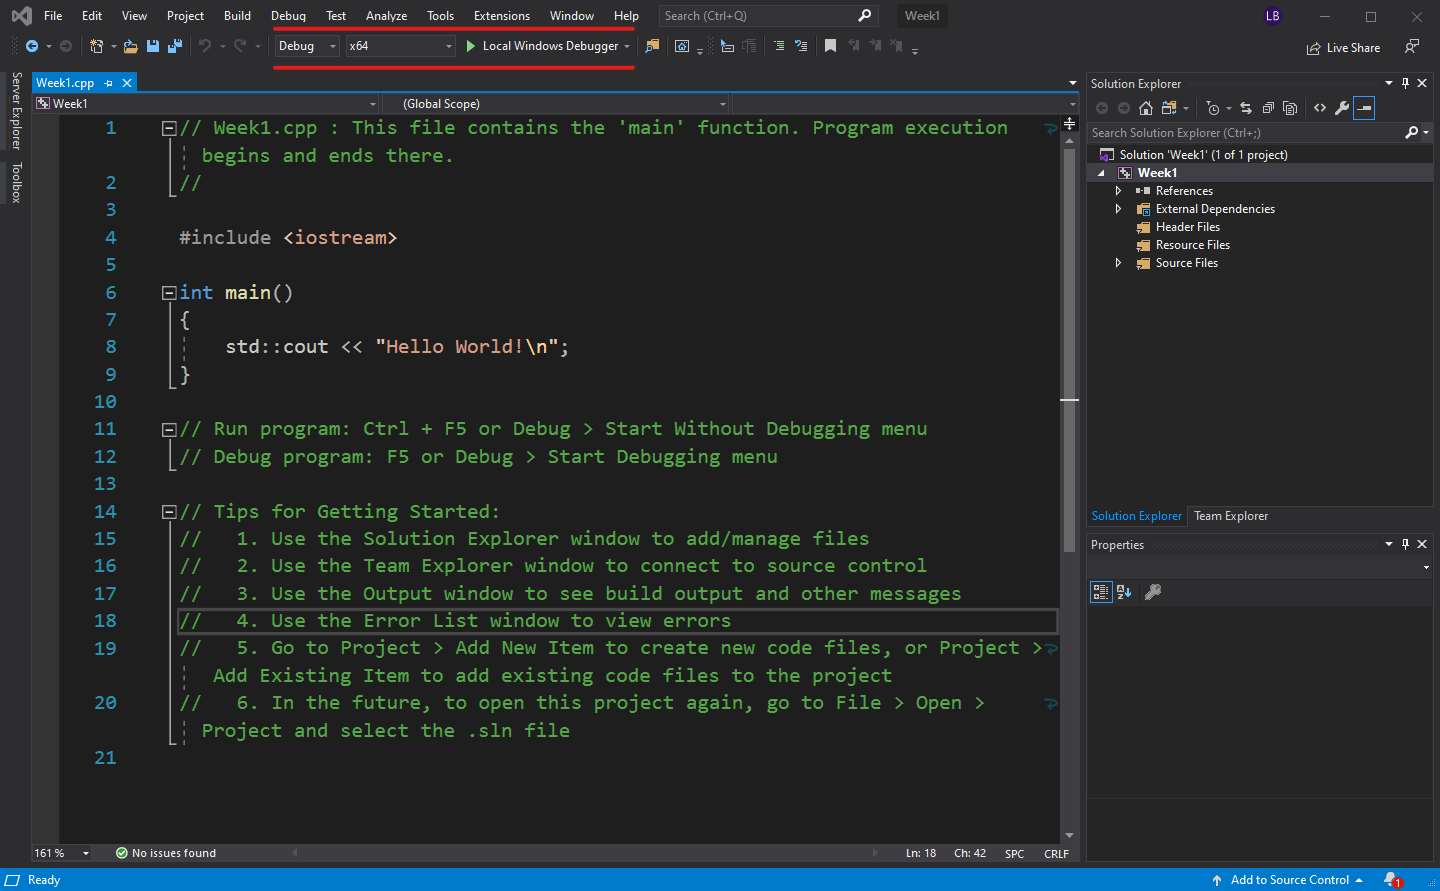
\includegraphics[width=0.8\textwidth]{img/new-hello-world.png}
      \caption{\label{helloworld} Running a program in Visual Studio}
  \end{figure}

  This action will open an output interface at the bottom, in which the output of compilation is shown.
  Once the build is complete, a console window should open containing the expected output, and Visual Studio will switch into the \textbf{Debugger} interface.
  This process might take some time on the first run, so do not be surprised if it takes a while to load and start the first time you compile and run.
  Note: If the code contains an error and is not well formed, Visual Studio will not run the code.

  \item You should see a new window opening with a colored rectangle. This is our application.
  It is not very interesting yet, so just close the window of the started program.
  \item We will now start to experiment by modifying the source code in the main window. First, open the file “\texttt{draw.c}” in the Solution Explorer.
  \item The file contains comments starting with the characters “\texttt{//}” that describe the behavior of the program. If you scroll down a few lines you find this code:
  \begin{lstlisting}
  // this "function" draws a rectangle
  void draw(int frame){
    // define the properties of the color used for the rectangle
    rgb_t color;
    color.red   = 255;
    color.green = 255;
    color.blue  = 0;

    // define the properties of the rectangle
    SDL_Rect rect1;
    rect1.x = 100; // coordinate x
    rect1.y = 200; // coordinate y
    rect1.h = 100; // height
    rect1.w = 100; // width
    // draw the rectangle with the given properties of the dimensions and color
    draw_rect(rect1, color);
  }
  \end{lstlisting}
  This code uses our concept of “Sequence” to run several instructions, one after the other, sequentially.
  It first defines a color (Lines 4-7) using the RGB color mode (0 means no color in the respective channel and 255 means maximum brightness).
  Then it defines the dimensions of a rectangle (Lines 10-14).
  Finally, it draws the rectangle by calling the “function” \func{draw\_rect} in Line 16.

  The variable \texttt{frame} contains a number that is incremented every time the image is re-drawn, which may be used to change the graphics over time.
  \item Experiment by changing some values in the code as you like and rerun the code to see the impact.
  Maybe change one of the fixed numbers to \texttt{frame}, too?
\end{steps}

\begin{literature}
\item Welcome to the Visual Studio IDE
\url{https://docs.microsoft.com/en-us/visualstudio/get-started/visual-studio-ide?view=vs-2019}
\item Tour of Visual Studio: \url{https://docs.microsoft.com/en-us/visualstudio/ide/quickstart-ide-orientation?view=vs-2019}
\end{literature}


\groupwork{Control Structures for Structured Programming}{40}

As part of this task, we will explore basic control structures in C that implement  \textbf{selection} and \textbf{iteration}.
We have already seen \textbf{sequence} in action because the program is executed step by step.

We will modify our little \func{draw} function in the same project that we used before, exploring several options.
There are several different ways you can achieve each goal. Please feel free to explore and play with the code.
Some steps are marked as \textbf{advanced}; only perform them if you feel comfortable.
The \textit{hints} section underneath provides some support.

\begin{steps}
\item Team up with one of your neighbors that has a similar skill level, and sit in front of one computer. (We will enquire about your skill level and organize the groups.)
\item Work through the following tasks: (time: 30 minutes)
  \begin{enumerate}
  \item First, modify the code so that the graphics change over time.
  To do this, we will use the variable \texttt{frame} that contains how often the image has been re-drawn.

  After some initial experimentation, think about how you could make the picture displayed alternate between two states every other frame.
  To do this, you can use the C construct for \textbf{selection}, which is illustrated in the following code:
\begin{lstlisting}
  if ( condition ){ // if condition != 0, then
    // run this code
  } else {
    // run this other code
  }
\end{lstlisting}
  So, you could create, for instance, code like this:
\begin{lstlisting}
  if ( 5 < 10 ){
    rect1.x = 100;
  } else {
    rect1.x = 200;
  }
\end{lstlisting}
Which means that if 5 is smaller than 10, which it is, then set the x coordinate of our rectangle to 100. The condition here is fixed but normally we use variables in the condition;
here, you want to do something with the variable \texttt{frame}.
Modify the if statement above to make the coordinates of the rectangle alternate between two locations depending on the frame.

  \item Try to move the rectangle from left to right (using the \texttt{frame} variable).
  Can you stop the rectangle from moving out of the window?
  \textbf{Advanced}: Can you make it bounce back and forth between the boundaries of the window?

  \item Next, try to create 5 rectangles and place them next to each other. (You can choose the layout.)
  This can be achieved using the \texttt{for} loop.
  Remember that this loop runs code for initialization, then checks the condition and, if it is true, runs the loop body. After each iteration, it runs the code in the iteration expression.

  The following example runs the loop body 5 times; the variable \texttt{i} can be used to distinguish the different iterations.
    \begin{lstlisting}
      for(int i=0; i < 5; i++){
        // loop body
      }
    \end{lstlisting}

  \item Modify your code from the previous step to give each rectangle a different color. That is, the first rectangle should have a different color than the next one and so on.

  \item Modify your code again and make the color vary depending on the frame.
  \textbf{Advanced:} You may see that the color is flickering. For example, if you modified the green channel, the rectangle might get more and more green and then black again.
  Can you change the code so that the color alternates; that is, it gets gradually more intense (say for 20 frames) and then gradually less intense again?

  \item Organize a 2D shape of 5x5 rectangles next to each other, each with a different color.
  \end{enumerate}
\item We will discuss the outcome of the practical in groups of 5-6 people. Reflect on the task: Where did you struggle? What did you learn? (5 minutes)
\item Group discussion: The lecturer will discuss the outcome of the practical with the class; potentially we will look at a program and discuss it.
If you feel comfortable, feel free to present one of your programs to the rest of the class.
\end{steps}

If you are already an experienced programmer and finish early you may check out the easter egg program.

\begin{hints}
  \item The following calculates the remainder of division by two: $5 \% 2$ (result is 1).

  \item The file “\texttt{src/code-snippets.c}” contains our base version of the code and potential solutions for each different step.
  In order to use them, replace the body of \func{draw} with the content of the respective step.
  \item The constant SIZE represents the width and height of the window.

  \item If you receive a compilation error referring to something called "SDL", check that you have opened the "Solution SpringProject" and not another C file.
\end{hints}

\subsection{Easter Eggs: A Bouncy Reading}

If you have time and feel comfortable with the groupwork, you could try some fun programs that can be easily derived from our example.

In the directory rectangle, you will find an example program with a moving logo that you can try.
The program \texttt{rectangle3.c}, for example, provides a logo that bounces from the corners and \texttt{rectangle-manual.c} allows you to control its movement using the arrow keys.

In order to use one of them, you must delete \texttt{code-snippets.c} and \texttt{draw.c} in the solution explorer.
Then you can add one of the C files as follows: Right click in the Solution Explorer on Source File. Select “Add”, then “Existing Item”.
Locate the rectangle directory and add one of the files.
Note that there can be only one of the rectangle examples used at a given time, as they are all complete programs.
Now you should be able to compile and run these programs.

\end{document}
